% ****** Start of file aipsamp.tex ******
%
%   This file is part of the AIP files in the AIP distribution for REVTeX 4.
%   Version 4.1 of REVTeX, October 2009
%
%   Copyright (c) 2009 American Institute of Physics.
%
%   See the AIP README file for restrictions and more information.
%
% TeX'ing this file requires that you have AMS-LaTeX 2.0 installed
% as well as the rest of the prerequisites for REVTeX 4.1
%
% It also requires running BibTeX. The commands are as follows:
%
%  1)  latex  aipsamp
%  2)  bibtex aipsamp
%  3)  latex  aipsamp
%  4)  latex  aipsamp
%
% Use this file as a source of example code for your aip document.
% Use the file aiptemplate.tex as a template for your document.
\documentclass[%
aip,pop,amsmath,amssymb,
%preprint,%
 reprint,%
%author-year,%
%author-numerical,%
]{revtex4-1}


\usepackage{color}
\usepackage{xcolor}
\usepackage{graphicx}% Include figure files
\usepackage{bm}% bold math
%\usepackage[mathlines]{lineno}% Enable numbering of text and display math
%\linenumbers\relax % Commence numbering lines

\newcommand{\subfigimg}[3][,]{%
  \setbox1=\hbox{\includegraphics[#1]{#3}}% Store image in box
  \leavevmode\rlap{\usebox1}% Print image
  \rlap{\hspace*{200pt}\raisebox{\dimexpr\ht1-2\baselineskip}{#2}}% Print label
  \phantom{\usebox1}% Insert appropriate spcing
}

\begin{document}

\preprint{AIP/123-QED}



\title[]{On the compressibility effect in test particle acceleration 
by magnetohydrodynamic turbulence}% Force line breaks with \\
\author{C.A. Gonz\'alez}
\author{P. Dmitruk}
\author{P.D. Mininni}
 \email{caangonzalez@df.uba.ar}
 \
\affiliation{Departamento de F\'isica, Facultad de Ciencias
Exactas y Naturales, Universidad de Buenos Aires, Argentina}
\author{W.H. Matthaeus}
\
\affiliation{Bartol - Department of Physics and Astronomy, University of Delaware, USA}


%\date{\today}% It is always \today, today,
             %  but any date may be explicitly specified

\begin{abstract}
The effect of compressibility in charged particle energization by 
magnetohydrodynamic (MHD) fields
is studied in the context of test particle simulations. 
This problem is relevant 
to the solar wind and the solar corona due to the compressible 
nature of those astrophysical 
scenarios. We consider turbulent electromagnetic fields obtained from  
direct numerical simulations 
of the MHD equations with a strong background magnetic field.  
In order to explore the compressibilty effect over the particle dynamics 
we performed
different numerical experiments: an incompressible case and two weak 
compressible cases, with 
Mach number $M=0.25$ and $M=0.1$. 
We analyze the behavior of protons 
and electrons in those turbulent fields,  which are well known to form 
aligned current sheets in 
the direction of the guide magnetic field. 
We show that compressibility enhance the 
efficiency of proton acceleration and that the energization 
is due to perpendicular electric 
fields generated between currents sheets. On the other hand, 
electrons remains magnetized and 
they show an almost adiabatic motion, and no effect of compressibility 
is observed.
%Valid PACS numbers may be entered using the \verb+\pacs{#1}+ command.
\end{abstract}

%\pacs{Valid PACS appear here}% PACS, the Physics and Astronomy
                             % Classification Scheme.
%\keywords{}%Use showkeys class option if keyword
                              %display desired
\maketitle

%\begin{quotation}
%The ``lead paragraph'' is encapsulated with the \LaTeX\ 
%\verb+quotation+ environment and is formatted as a single paragraph before the first section heading. 
%(The \verb+quotation+ environment reverts to its usual meaning after the first sectioning command.) 
%Note that numbered references are allowed in the lead paragraph.
%
%The lead paragraph will only be found in an article being prepared for the journal \textit{Chaos}.
%\end{quotation}

\section{\label{sec:level1}INTRODUCTION:}
Turbulence is an ubiquitous phenomenon in many astrophysical 
environments in which a wide  
variety of temporal and spatial scales are involved. This is the case of 
the solar wind or the 
intellestar medium where the energy is transported from 
large to small scales up to 
kinetic scales where the energy is dissipated. 
Turbulence is the result of the  non linear 
interaction between fluctuations of the velocity and magnetic fields, 
leading to a 
spatial intermittency that is associated with coherent structures,
 where the dissipation is 
concentrated in strong gradient regions that impacts on the heating, 
transport and particle 
acceleration in plasma \cite{M1}.

The efficiency of MHD turbulence to accelerate charged particles 
and its importance in space 
physics has been reported by many different authors\cite{F1,L1,M2}, 
but the great variety of 
scales involved in turbulence and the particle dynamics
makes this problem a big challenge.
On long timescales (large eddy turnover times), dynamics is
governed by stochastic acceleration and momentum diffusion is
the main acceleration 
mechanism which has been mainly applied for cosmic-ray energization 
studies and frequently
addressed by quasi-linear theory (QLT)\cite{S1,CH1,Lange1}. 
In diffusion studies 
MHD turbulence is commonly represented as a random 
collection of waves, and that 
representation lacks of coherent structures that has an important role 
at particle scales\cite{Vlahos}

Dmitruk et al 2004\cite{PD1}, 
using test particle simulations in static electromagnetic fields, obtained 
from direct 
numerical simulation (DNS) of MHD equations, showed that particle 
energization at dissipation
scale is due to current sheets and the acceleration mechanism 
depends on the particle 
gyroradii. 

Using a more sophisticated model, but still static turbulent 
electromagnetic fields, Dalena et 
al 2012.\cite{Dalena2012} shows essentially the same results.
Electrons initially moving with 
Alfv\'en velocity experience parallel (to the guide magnetic field)
acceleration by 
parallel electric fields inside current sheet chanels. 
On the other hand, protons are accelerated in a two stage process: 
initially they are parallel accelerated and gain substantial energy 
in a short time. Then, when the proton gyroradius becomes
comparable with current sheet thickness,
it is accelerated perpendicularly to the guide field.  


Effects of compressible MHD on particle energization has been reported 
in diffusion studies\cite{Chandran2003,CHO1}, where supersonic
turbulence was considered.

There are also reports of test particle pitch angle scattering in 
MHD turbulence, Lynn et al 2013\cite{Lynn2013}, considering 
second order Fermi acceleration by weak compressible MHD running simultaneously
the test particle and MHD fields, and imposing a scattering rate.
It is found that compressibility 
is an important effect to produce non-thermal particles. 

Additionally, there are
studies where test particles and fields are simultaneously resolved.
Weid et al 2015\cite{Weidl2015} and Teaca et al. 2014\cite{Bogdan2014}, 
use an incompressible MHD model, analyzing the effect of the 
correlation between magnetic and velocity fields 
on pitch-angle scattering and particle 
acceleration. They found that imbalanced turbulence (nonzero cross-helicity in 
the system) enhances the particle acceleration and also 
the pitch angle scattering.

In the present work we are interested in the compressibility effect 
on particle 
acceleration by coherent structures corresponding to a direct numerical 
simulation of the MHD equations, fixing the the fields which accelerate
the particles. 
We 
analyze the particle behavior for three different situations: an 
incompressible case, and 
two weak compressible cases changing the sound Mach number value. 

The organization of this paper is the following:  In section 2  
we describe the model 
employed in our investigation, the equations and properties of 
turbulent MHD fields and the 
test particle model including the parameters that correlate 
particles and fields; 
in section 3 we show the properties of proton and electron dynamics 
and in section 4, we
discuss about our findings.

\begin{figure*}[<t>]
\begin{center}
{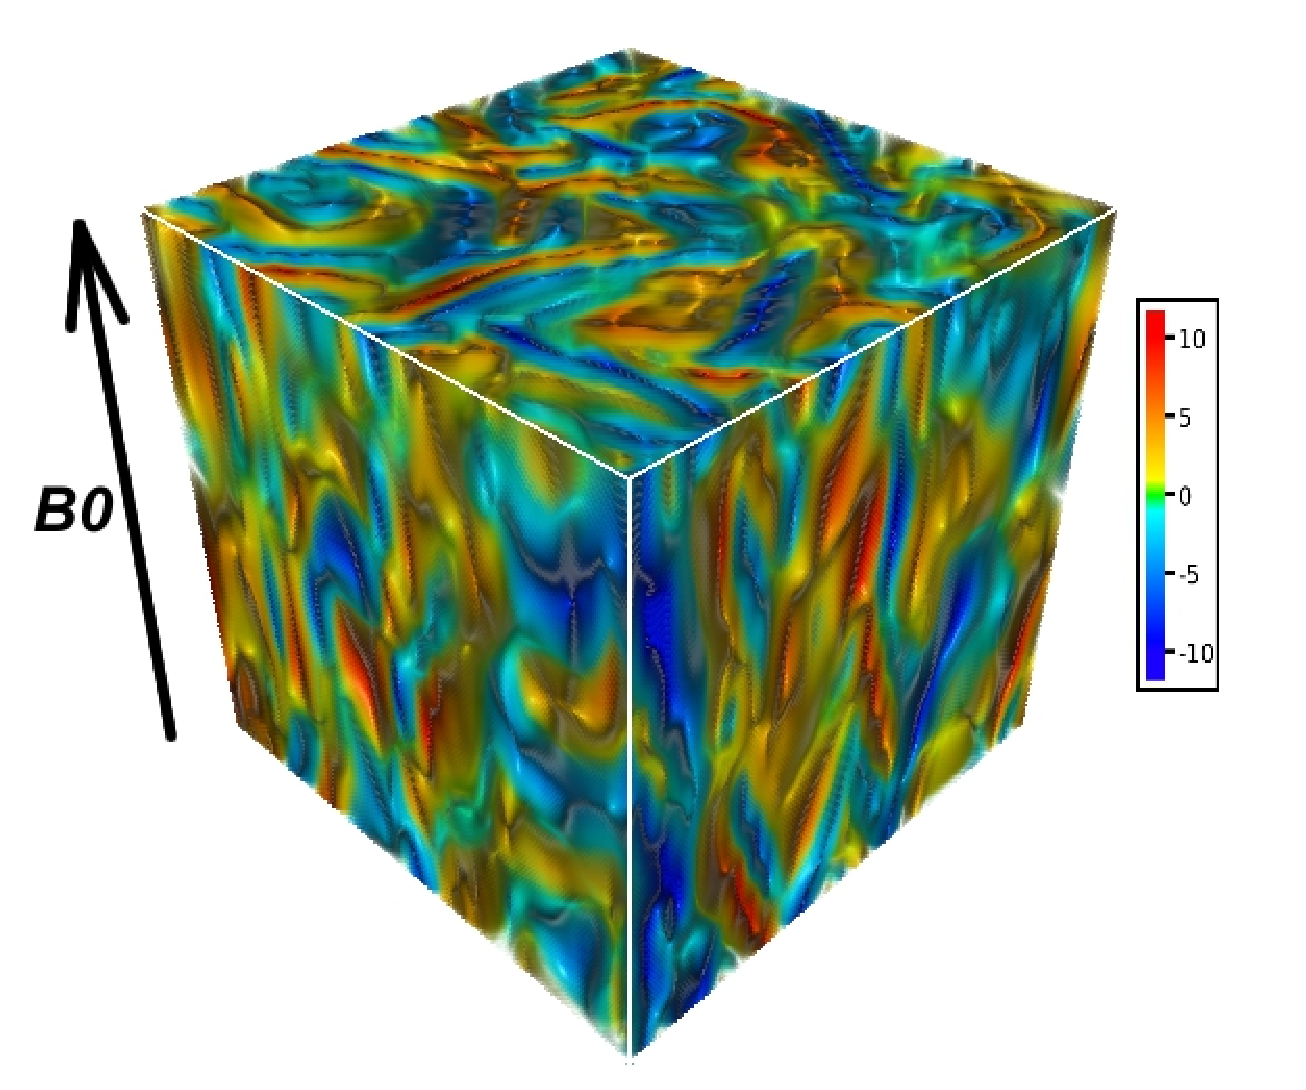
\includegraphics[width = 0.45\textwidth]{./Figures/Fig1_a}}
{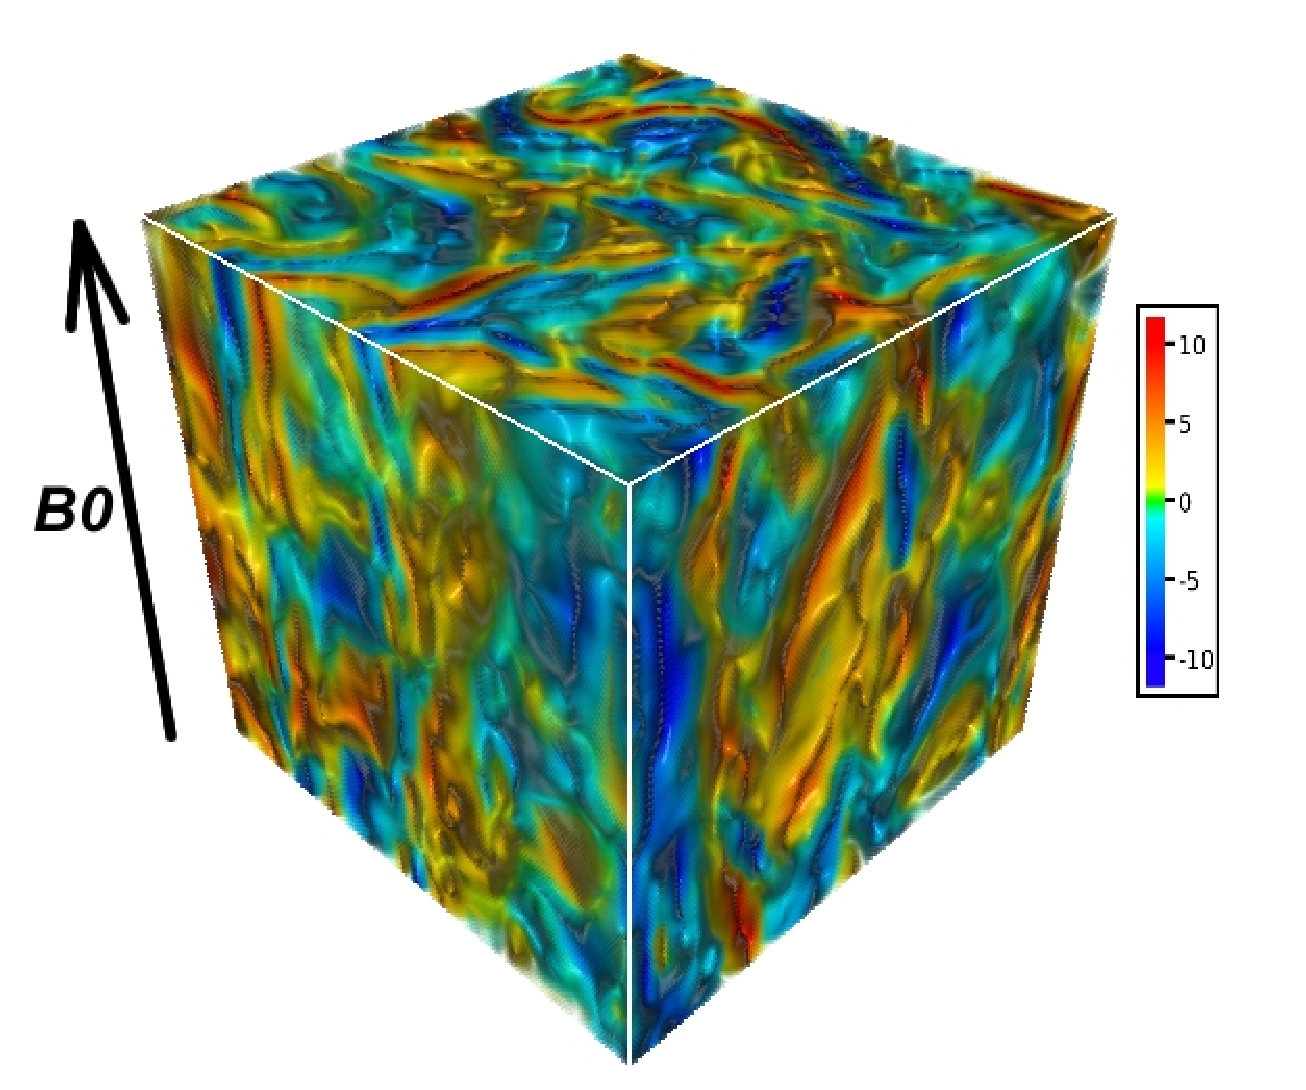
\includegraphics[width = 0.45\textwidth]{./Figures/Fig1_b}}
\caption{Three dimensional view of the parallel current density $J_z(x,y,z)$. (Left) Incompressible and 
(Right) Compressible field with Mach number $M=0.25$ case at $t/t_0 =2$.}
\end{center}
\end{figure*}


\section{\label{sec:level2}MODEL:}
The macroscopic description of a plasma is given by the three-dimensional compressible MHD equations: the continuity (density) equation, the equation of motion, the magnetic field induction equation, and the equation of state (1-4) respectively, which involves fluctuations  of the velocity field $\textbf{u}$, magnetic field $\textbf{b}$ and density $\rho$. We assume a large-scale background magnetic field $B_0$ in the z-direction, so the total magnetic field is $\mathbf{B = B_0 + b}$


\begin{equation}
 \frac{\partial \rho}{\partial t} + \nabla \cdot (\textbf{u}\rho) = 0
\end{equation}

\begin{equation}
 \frac{\partial \textbf{u}}{\partial t} + \textbf{u} \cdot \nabla \textbf{u} = - \frac{\nabla p}{\rho} + \frac{\textbf{j} \times \textbf{B}}{4\pi\rho} 
 + \nu \left( \nabla^2 \textbf{u} +    \frac{\nabla \nabla \cdot \textbf{u} }{3} \right)
\end{equation}

\begin{equation}
\frac{\partial \textbf{B}}{\partial t} = \nabla \times (\textbf{u} \times \textbf{B}) + \eta \nabla^2 \textbf{B}
\end{equation}

\begin{equation}
 \frac{p}{\rho^{\gamma}} = cte
\end{equation}


Here $p$ is the pressure, $\nu$ the viscosity, $\eta$ the magnetic 
diffusivity and
$\textbf{J}=\nabla \times \textbf{B} $ is the current density. 
We assume a polytropic 
equation of state $p/p_0= (\rho/\rho_0)^{\gamma}$, with $\gamma=5/3$, and
$p_0, \rho_0$ the equilibrium (reference) pressure and density. 
We consider two weak compressible cases with Mach number
($M= \sqrt{\gamma p/\rho}$) equal to $M=0.25$ and $M=0,1$. Additionally, 
in order to 
have a reference to measure the effect of compressibility on particle 
acceleration, we consider an
incompressible case (with $\nabla \cdot \textbf{u} = 0$).

The magnetic and velocity fields are here expressed in Alfv\'en speed units; 
a characteristic 
plasma velocity is given by the parallel Alfv\'en wave velocity
along the mean magnetic 
field $v_A = B_0/\sqrt{4\pi\rho_0}$. An Alfven speed based on field 
fluctuations can also be defined as $v_0=\sqrt{<b^2>/4\pi\rho_0}$. 
We take $v_0$ as a unit for velocity and magnetic field fluctuations. 

We use the turbulence correlation length $L$ as unit length. 
The unit timescale $t_0$
is derived from the unit length and the Alfven speed $t_0=L/v_0$.

The MHD equations are solved numerically using 
a Fourier pseudospectral method with periodic 
boundary conditions in a cube of size  $L_{box}=2\pi L$; 
this scheme ensures exact energy 
conservation for the continuous time spatially discrete equations. 
The discrete time 
integration is done with a high-order Runge-Kutta method and a
resolution of ($256^3$) 
Fourier modes is considered. For the kinematic Reynolds number 
$R=v_0L/\nu$ and magnetic Reynolds
numbers $R_m=v_0L/\eta$, 
we take $R=R_m= 1000$, which are limited here by available
spatial resolution. We consider a decaying simulation from an 
initial state with the kinetic 
and magnetic field fluctuations populating an annulus in Fourier k-space 
defined by a range of wavenumbers with
$ 3\leq k \leq4$, constant amplitudes and random phases.

When the turbulence is fully-developed a broad range of 
scales develops, from outer scale $L$ to 
dissipation scale $l_d\approx L/32$. We then consider this
turbulent (fixed) MHD state to push the test
particles.

The behavior of a test particle in an electromagnetic field 
is described by 
the nonrelativistic particle equations of motion:

\begin{equation}
  \frac{d\textbf{v}}{dt} = \alpha(\textbf{E} + \textbf{v} \times \textbf{B}), \ \ \ \  \frac{d\textbf{r}}{dt} = \textbf{v}
\end{equation}
 
The nondimensional electric field \textbf{E} is obtained from Ohm's law 
normalized with $E_0= v_0 B_0/c$ as follows:

\begin{equation}
 \textbf{E} =  -\textbf{u}  \times \textbf{B} + \frac{\textbf{j}}{R_m} 
\end{equation}

The adimensional parameter $\alpha$ relates particles and MHD field parameters:

\begin{equation}
\alpha=Z\frac{m_p}{m}\frac{L}{\rho_{ii}}
\end{equation}
Where $\rho_{ii}$ is the proton inertial length given 
by $\rho_{ii}=m_pc/(e\sqrt{4\pi\rho_0})$. The $\alpha$ parameter also 
represents the nominal 
particle gyroradii and measures the range of scales involved in the system.
One could expect a value
$\alpha \gg 1$ specially for space physics and astrophysical plasmas.
This represent a huge computational challenge due to 
numerical limitations. 
We consider here a dissipation length scale
$l_d=L/32$ as stated above, which is also of the order of
the current sheet thickness.

In the fixed MHD turbulence state, $10000$ test particles are 
randomly distributed 
in the computational box and the equation of motion of particles 
subject to the MHD
electromagnetic field are solved using a high-order Runge-Kutta method. 
Furthermore, 
we use linear interpolation for field values on each particle position.


Particles are initialized at rest but in a short time, they
acquire a Gaussian velocity distribution function with a 
root mean square (rms) value of the order of the Alfven velocity, 
as discussed in Dalena et al. 2012.
It is
well known that the particle gyroradius determines the acceleration 
process and our aim in 
this paper is to explore the compressibility effect on 
acceleration of large and small particle 
gyroradii. In the next section we show two diferent compressible cases 
with Mach number $M=0.25$ and $M=0.1$ 
and an incompressible case. In all the cases the mean magnetic field
is set to $B_0=10$. We present the behavior of protons with a 
nominal gyroradius $1/32$ and electrons  ($m_e=m_p/1836$)
with nominal gyrodadius $1/58752$.


\section{\label{sec:level3}RESULTS:}

In Figure 1
a three-dimensional view of the z-component current density $J_z(x,y,z)$
is shown at
$t=2t_0$ for an incompressible case and a compressible case with $M=0.25$.
It is 
observed that current sheets are aligned in the direction of 
the guide magnetic field. 
It can be seen that in both cases the structures are similar 
but more corrugated in the 
compressible case and smoother in the incompressible one. It is worth
mentioning that we used the same 
initial conditions for all the simulations. 
Coherent structures like
this show the natural tendency of the MHD equations to 
develop strong gradients
leading to many reconection zones, which
is well known to be one of the mechanisms behind the charged particle
acceleration.

Figure 2 shows the total spectrum of kinetic (top) and magnetic field (bottom) 
for 
the compressible $M=0.25$, $M=0.1$ cases and the
incompressible case. At the inertial range
there are almost no differences between compressible and incompressible 
energy spectra for 
both magnetic and velocity fields, although slightly more energy at 
large scales is observed in the incompressible case.
On the other hand, at wavenumbers beyond the dissipation scale 
(that is, $k\geq32$),  an excess of energy is observed 
as the Mach number is increased.  
This feature is more evident for the kinetic energy spectrum
than magnetic energy spectrum. Since protons 
are mostly interacting with structures at that size this could be an 
important effect on proton acceleration.


\begin{figure}[h!]
\begin{center}
{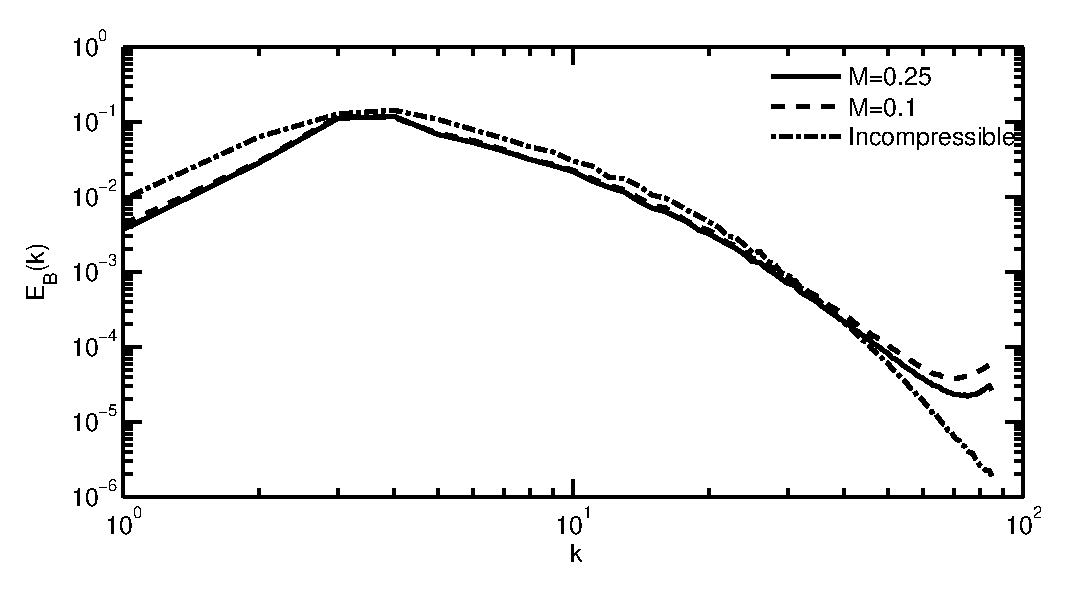
\includegraphics[width = 3in]{./Figures/Fig2_b}}\\
{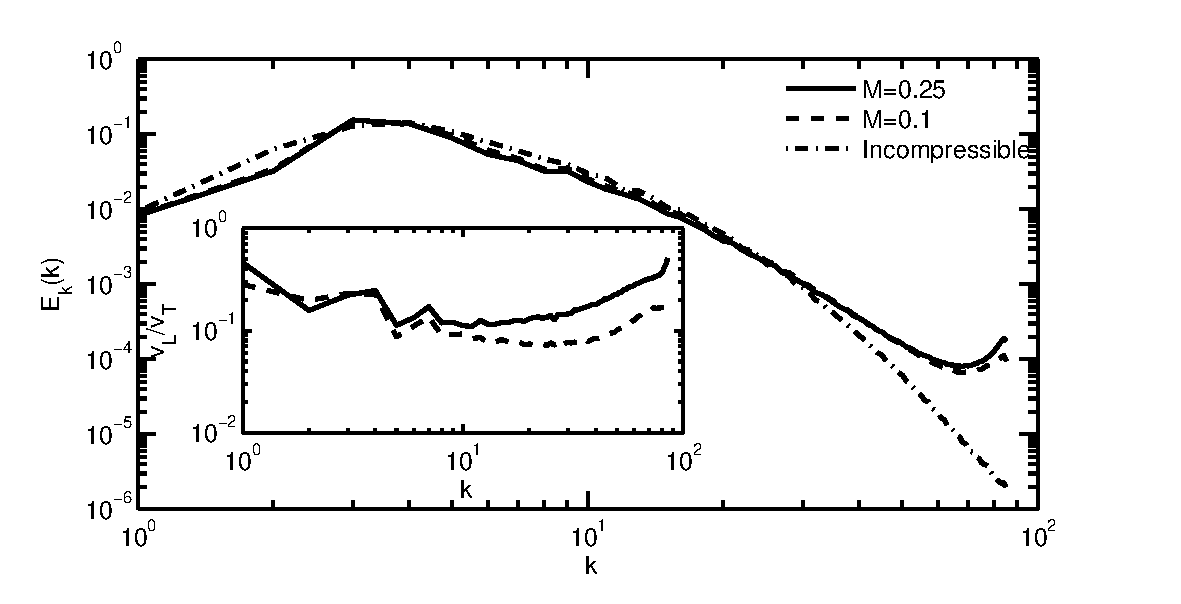
\includegraphics[width = 3in]{./Figures/Fig2_a}}
\caption{(Top). Total kinetic energy spectrum for compressible case with Mach 
number $M=0.25$ (solid line), $M=0.1$ (dashed line) and incompressible case 
(dashed-dot line).
(Bottom) Total Magnetic energy spectrum for the three cases named 
before using the same line 
type.}
\end{center}
\label{mean square velocity}
\end{figure}

Figure 3 shows the time evolution for the mean value of
the perpendicular $v_\perp=\sqrt{v_x^2+v_y^2}$ 
(top) and parallel $v\parallel=v_z$ (bottom) proton velocity 
for the compressible $M=0.25$, $M=0.1$ cases
and the incompressible case. 
The typical acceleration process observed in previous studies is
evident, proton are accelerated perpendicularly with respect to $B_0$, 
and they are less
parallel accelerated. 

Moreover, the compressibiliy effect on particle acceleration 
is clearly observed.
Protons are highly accelerated as compressibility of the fluid increases 
for both perpendicular and parallel directions.
Acceleration of protons is also observed in the 
incompressible case (see inset plot) but
the value reached at the end of the simulation is much lower than in both
compressible cases, even with a relatively small value of the 
Mach number $M$.

\begin{figure}[h!]
\begin{center}
{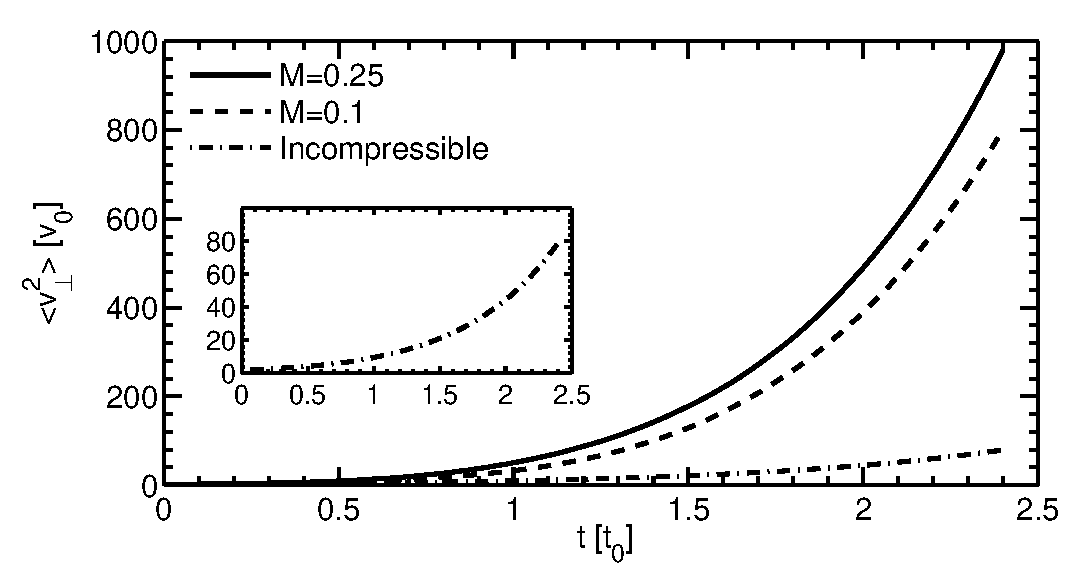
\includegraphics[width = 3.5in]{./Figures/Fig3_a}}
{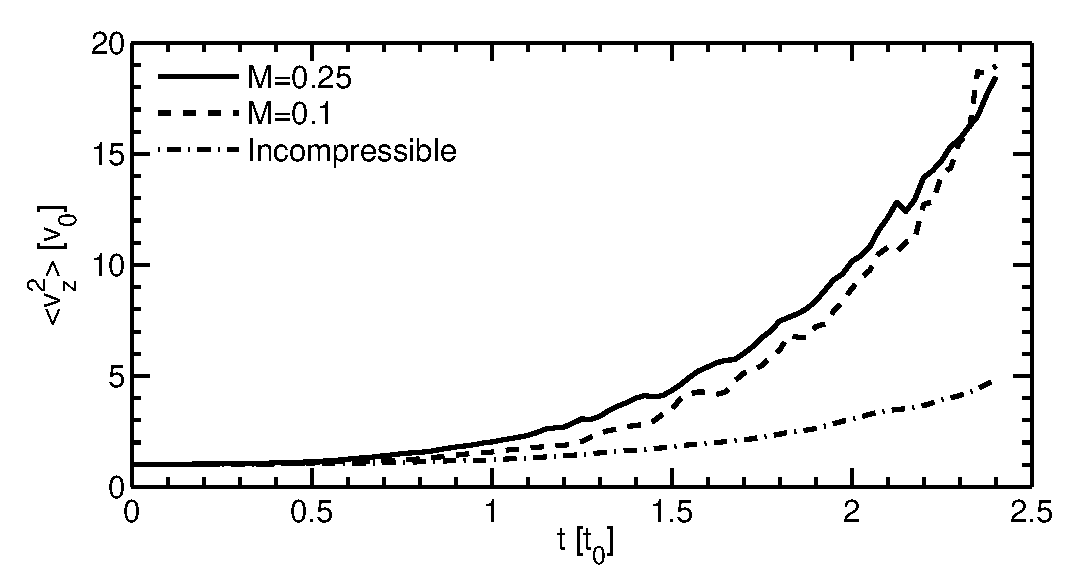
\includegraphics[width = 3.5in]{./Figures/Fig3_b}}
\caption{Particle mean square velocity as function of time: (Left)
Proton perpendicular velocity $v_\perp = \sqrt{v_x^2 + v_y^2}$ 
for two different Mach number
cases, $M=0.25$ (solid line), $M=0.1$ (dashed line) and the
incompressible case (dash-dot line). 
(Right) Proton parallel velocity $v\parallel=v_z$ for $M=0.25$, $M=0.1$ 
and incompressible case with the
same line type.}
\end{center}
\label{mean square velocity}
\end{figure}

Figure 4 shows the probability distribution function (PDF) of the
perpendicular x-component (top) and the parallel z-component (bottom) 
of the electric field 
for the compressible and incompressible cases. 

The PDF shows that, as compression increase, long tails in the 
distribution arise and higher values of the perpendicular electric field 
are achieved.
Additionally the core part of the distribution function for the incompressible 
case is
thicker than the compressible cases.

\begin{figure}
\begin{center}
{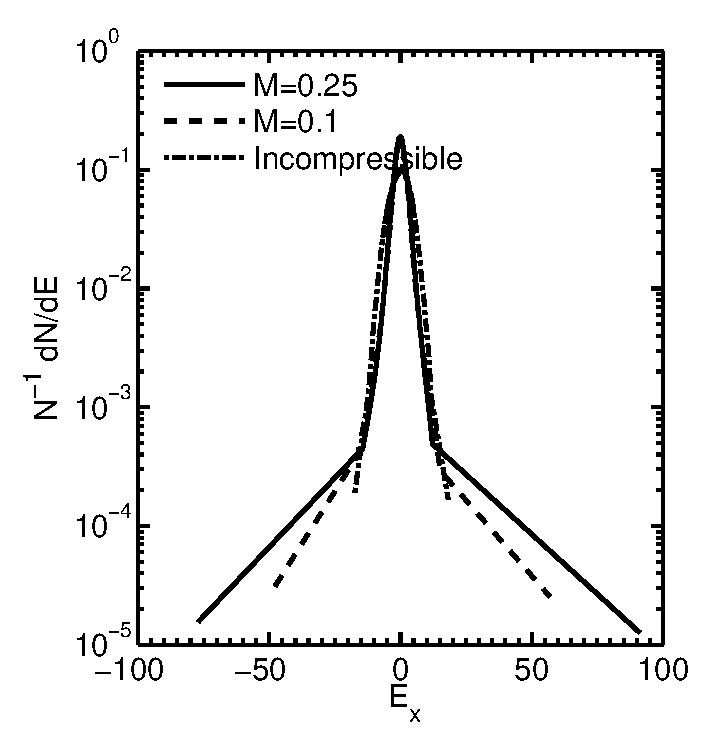
\includegraphics[width = 3in]{./Figures/Fig4_b}}
{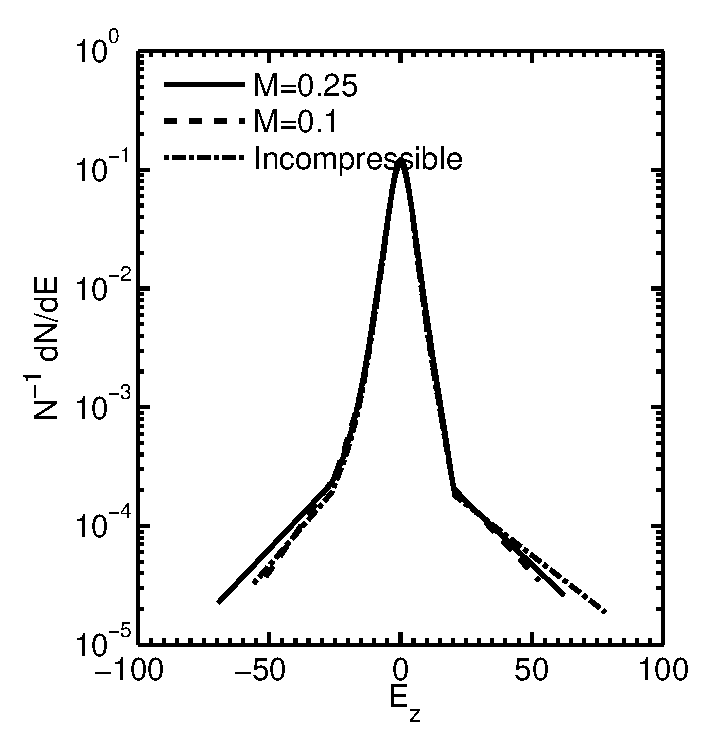
\includegraphics[width = 3in]{./Figures/Fig4_2}}
\caption{Probability density function of electric field components 
in the simulation box. 
(Left) perpendicular x-component 
for $M=0.25$ (solid line), $M=0.1$ (dashed line) and incompressible 
(dash-dot line). (Right) parallel z-component of electric field 
using the same line types.}
\end{center}
\label{mean square velocity}
\end{figure}
On the other hand, the PDF of the parallel electric field in the system shows 
that there is not
effect of compression.

In order to better understand the dynamics of protons, in Figure
5 we show the current density $J_z(x,y,z)$ together
with the trajectory of one of the most energetic protons,
for the compressible $M=0.25$ case.
It is observed that on the surrounding of the particle trajectory 
there are many current sheets, wich
may contribute to the proton energization.

\begin{figure}[h!]
\begin{center}
{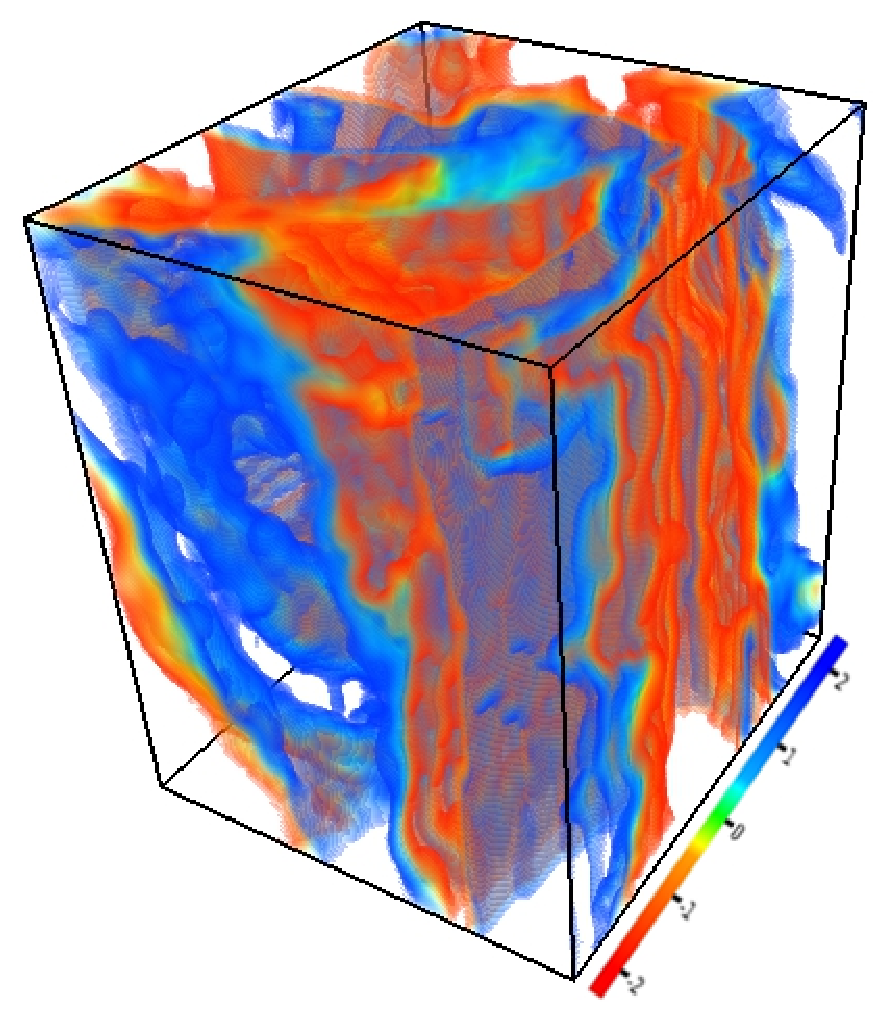
\includegraphics[width = 3in]{./Figures/Fig5_a}}
{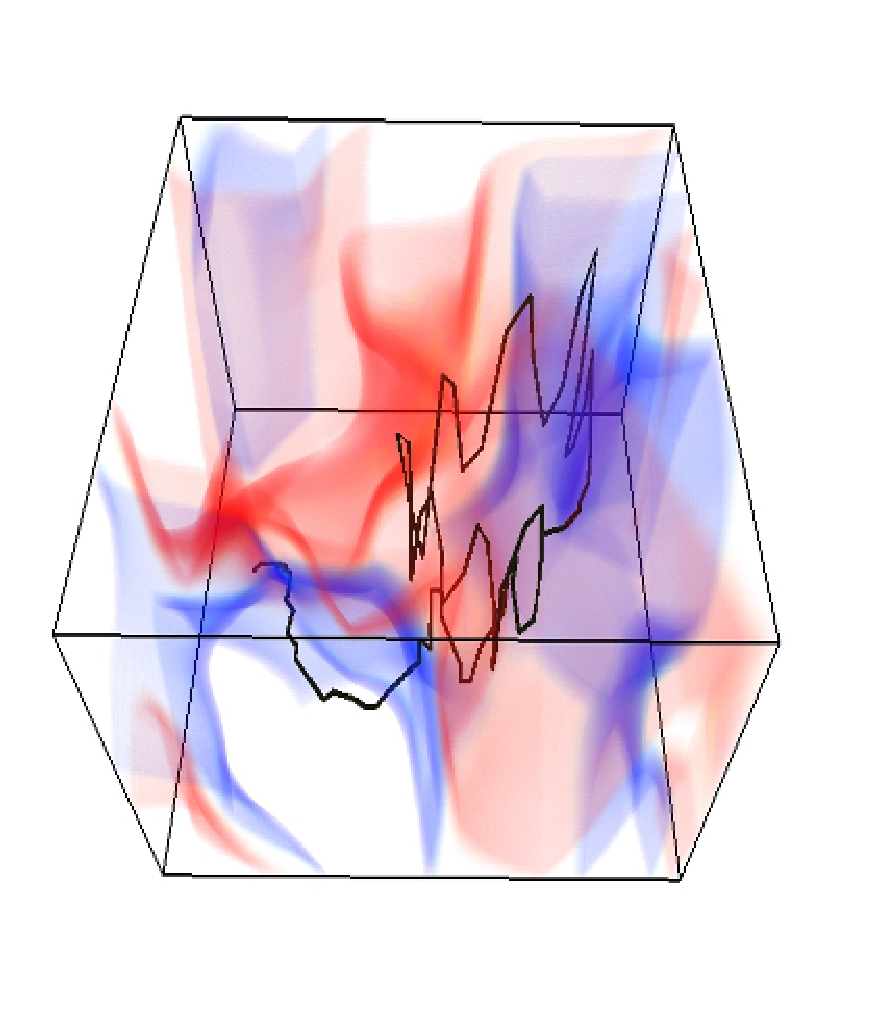
\includegraphics[height=2.87in, width = 3in]{./Figures/Fig5_b}}
\caption{(Left)View of the parallel current density $J_z(x,y,z)$;
(Right) Trajectory of one of the most energetic protons.}
\end{center}
\label{mean square velocity}
\end{figure}

\begin{figure*}[h!]
  \centering
  \begin{tabular}{@{}p{0.45\linewidth}@{\quad}p{0.45\linewidth}@{}}
    \subfigimg[width=\linewidth]{a)}{./Figures/Fig6_a_compress} &
    \subfigimg[width=\linewidth]{a)}{./Figures/Fig6_a_incompress} \\
    \subfigimg[width=\linewidth]{b)}{./Figures/Fig6_b_compress} &
    \subfigimg[width=\linewidth]{b)}{./Figures/Fig6_b_incompress} \\
    \subfigimg[width=\linewidth]{c)}{./Figures/Fig6_c_compress} &
    \subfigimg[width=\linewidth]{c)}{./Figures/Fig6_c_incompress} \\
    \subfigimg[width=\linewidth]{d)}{./Figures/Fig6_d_compress} &
    \subfigimg[width=\linewidth]{d)}{./Figures/Fig6_d_incompress}
  \end{tabular}
  \caption{(a) Parallel current density, 
(b) three components of the electric field, 
(c) velocity components, 
and (d) rms displacement as function of time for the most energetic particle:
(Left) compressible $M=0.25$ case and (Right) incompressible case}
\end{figure*}

\clearpage

Figure 6 shows the values of quantities following the trajectory of the
most energetic proton, that is the most energetic proton is identified
and the values of several quantities on the trajectory of this proton
are obtained: (a) the current density $J_z$
(b)electric field components $E_x, E_y, E_z$
(c) proton velocity components $v_x, v_y, v_z$
(c),root mean square displacement of the proton.
The panels on the left correspond to the compressible $M=0.25$ case
and the panels on the right correspond to the incompressible case.


It is observed that when there is a change of the sign in the 
current density $J_z$, there is also an increment in the 
perpendicular components of electric field that 
the particle experience and concurrently there is an increment 
of proton velocity. This situation
is repeatedly observed in time and the energy of proton increases.

A possible explanation for the change of sign in the current density is 
that the particle is entering and leaving two neighboring 
current sheets with different polarities while experiencing
a strong perpendicular electric field between those current sheets. 
The electric field
is stronger as the compression of the fluid increases (this can be noticed
by comparing panels on the left and right of Figure 6).
Consequently the velocity increment is larger in the compressible case 
than in the incompressible case.
This situation can be 
generalized for many particles in the simulation, 
resulting in the increase of the root mean 
square velocity for the ensemble of particles. 

\begin{figure}[<t>]
\begin{center}
{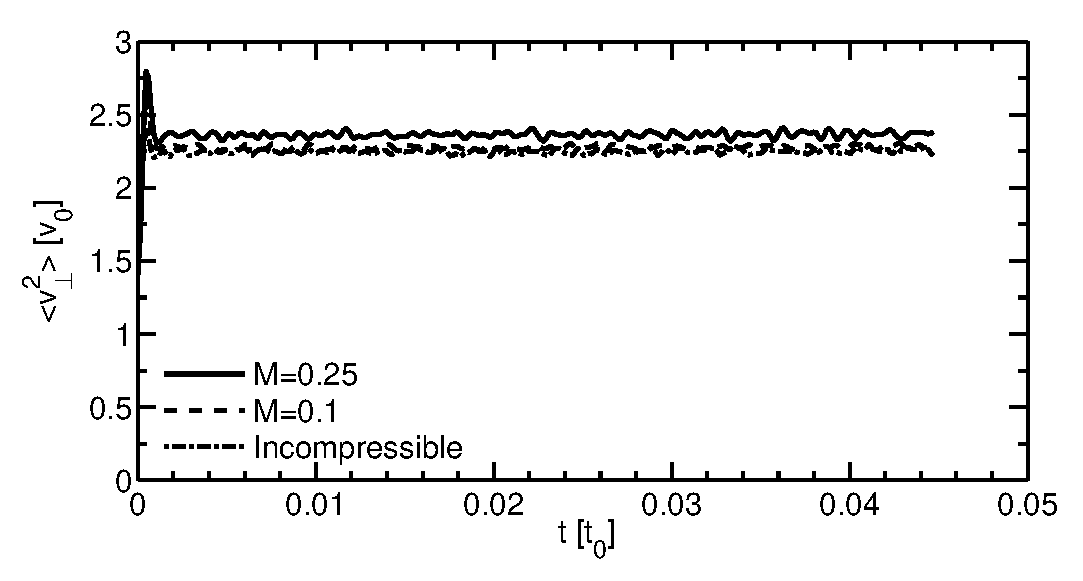
\includegraphics[width = 3.5in]{./Figures/Fig7_a}}
{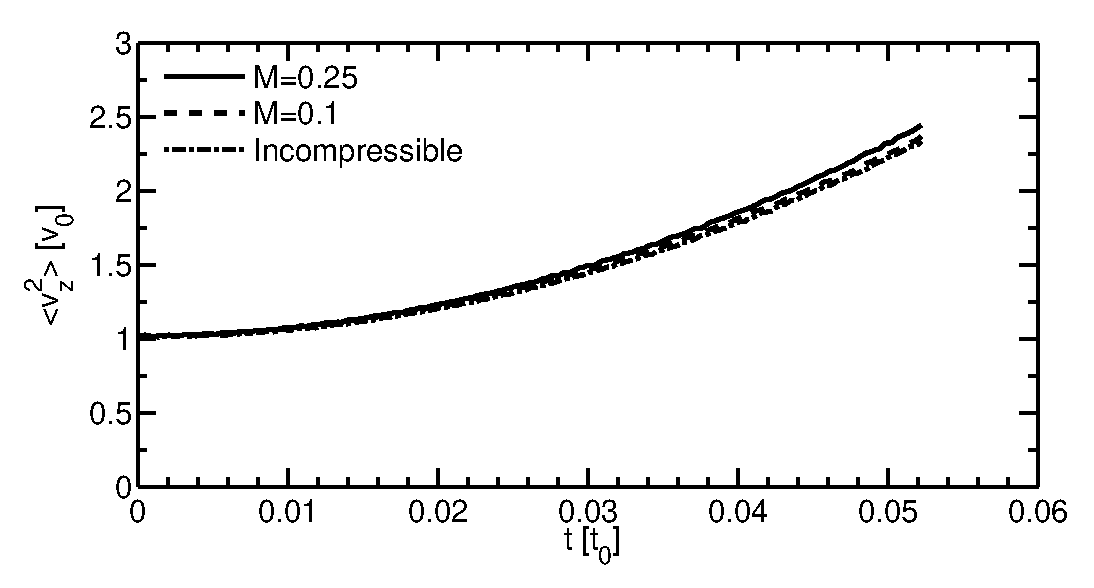
\includegraphics[width = 3.5in]{./Figures/Fig7_b}}
\caption{(Left) Time evolution of the perpendicular rms velocity for
electrons, for the compressible cases $M=0.25$ (solid line), 
$M=0.1$ (dashed line)
and the incompressible case (dot-dashed line); (Right) time evolution of
tha parallel rms velocity for electrons, using the same notation.} 
\end{center}
\label{mean square velocity}
\end{figure}

Figure 7 shows the time evolution for the perpendicular (top) 
and z-component (bottom) of electron
rms velocity for the compressible $M=0.25$, $M=0.1$ and incompressible cases.

It should be mentioned that we are showing
a short time simulation of electrons here.
This is due to limitation of computational resources, since electrons
requiere a small time step (to represent a physical 
small gyroradius).  The total time reached in the electron simulations
is of the order of almost 3000 
electron gyroperiods. 

Electrons present 
the typical parallel
energization reported in previous works. 
Besides there is no evidence that compression of 
the MHD fields enhance the electron acceleration and electrons gain 
almost the same energy
regardless the compressible level of the fluid.

Also, the
perpendicular rms velocity shows that electrons are initially accelerated 
but quickly exhibit a constant perpendicular energy. Constant 
perpendicular energy is consistent with the almost magnetic momentum 
conservation, 
which 
is one of the adiabatic invariants in charged particles dynamic in a magnetic 
field.

Since the gyradius of electrons is smaller than any of the length
scales structures 
in the fields, when electrons find a current sheet they travel 
along magnetic
field lines and there is not so much 
difference between compressible and incompressible cases.

It is important to remark that in longer timescales, of the order 
of many turnover times, 
electrons could obtain very high parallel energy, the motion is not 
almost adiabatic anymore and electrons
can reach other regions and interact with 
structures that generate other possible acceleration mechanisms, like pitch 
angle-scattering, betatron acceleration and others.

\section{\label{sec:level4}DISCUSSION:}
We have investigated the effect of compressible MHD turbulence 
on particle energization,
using test particle simulations in frozen electromagnetic fields obtained 
from direct numerical solutions of the MHD
equations. We have noticed that compression affects only the energization 
of large particle
gyroradius of the order of the dissipation length and no effect 
of compression for
small particle gyroradius is observed. 

Protons are accelerated by the perpendicular electric field 
generated on the interface of
current sheets and they gain substantial energy as they encounter 
these structures. 
Moreover the perpendicular electric field between current sheets 
is greater as compression
of the fluid increases leading to a higher proton acceleration. 

On the other hand, small particle gyroradii keep magnetized 
and gain parallel energy as 
they travel along magnetic field lines almost aligned with $B_0$.
No compression effect is
noted for these kind of particles and this is because the compressible modes 
in 
magnetohydrodynamics are perpendicular propagation modes ($k \perp B_0$) 
and then no
difference in the parallel electric field obtained from static MHD fields is presented.

In this paper we analyze the case of weak compressible turbulence 
despite the solar wind
and other astrophysical scenarios could be strongly compressible ($M \geq 1$), 
further we
showed that at least for low Mach number, compression could enhance 
the particle
energization by coherent structures and it has important implication 
in the study of
particle acceleration by turbulent fields.

In the incompressible case, which is the limit of infinit sound waves 
velocity, we 
observed that protons could be accelerated but less than in the compressible 
case.
The incompressible case serves as a reference to measure the influence of
compression on particle 
acceleration. Also the incompressible case could represent 
a real physical scenario, like fast
solar wind, which could accelerate particle as well.

\nocite{*}
\bibliographystyle{unsrtnat}
\bibliography{aipsamp}% Produces the bibliography via BibTeX.


\end{document}
%
% ****** End of file aipsamp.tex ******
